%mm substantive Mac Low changes marked so.  Minor changes done silently.

\documentclass[twocolumn]{aastex62}

% \submitjournal{ApJ}

\shortauthors{Beane et al.}
\shorttitle{The Galactic Midplane is Not a Plane}

\usepackage{graphicx}
\usepackage{gensymb}
\usepackage{bm}
\usepackage{mathtools}

\newcommand{\Gus}[1]{\textcolor{red}{#1}}

\newcommand{\Msun}{\ensuremath{\text{M}_\odot}}
\newcommand{\pc}{\text{pc}}
\newcommand{\kpc}{\text{kpc}}
\newcommand{\Myr}{\text{Myr}}
\newcommand{\Gyr}{\text{Gyr}}
\newcommand{\kms}{\text{km}/\text{s}}
\newcommand{\actunit}{\text{kpc}\,\kms}

\newcommand{\unit}[2]{\ensuremath{\textrm{#1}^{\mathrm{#2}}}}

\newcommand{\mi}{\texttt{m12i}}
\newcommand{\mf}{\texttt{m12f}}
\newcommand{\mm}{\texttt{m12m}}

\newcommand{\sgra}{Sgr~A\textsuperscript{*}}

\newcommand{\abs}[1]{\left| #1 \right|}
\newcommand{\avg}[1]{\left< #1 \right>}
\newcommand{\z}{z_r}
\newcommand{\uth}{\textsuperscript{th}}
\newcommand{\n}{\text{n}}

\newcommand{\beq}{\begin{equation}}
\newcommand{\eeq}{\end{equation}}

\newcommand{\thincolor}{pink}
\newcommand{\thickcolor}{brown}
\newcommand{\halocolor}{blue}

% affiliations
\newcommand{\cca}{Center for Computational Astrophysics, Flatiron Institute,
162 5th Ave., New York, NY 10010, USA}
\newcommand{\penn}{Department of Physics \& Astronomy, University of
Pennsylvania, 209 South 33rd St., Philadelphia, PA 19104, USA}
\newcommand{\amnh}{Department of Astrophysics, American Museum of Natural
History, Central Park West at 79th St., New York, NY 10024, USA}
\newcommand{\columbia}{Department of Astronomy, Columbia University, 550 W
120th St., New York, NY 10027, USA}
\newcommand{\victoria}{Department of Physics \& Astronomy, University of
Victoria, 3800 Finnerty Rd., Victoria, BC, V8P 4HN, Canada}
\newcommand{\nyuphys}{Center for Cosmology and Particle Physics, Department of
Physics, New York University, 726 Broadway, New York, NY 10003, USA}
\newcommand{\nyucds}{Center for Data Science, New York University, 60 Fifth
Ave., New York, NY 10011, USA}
\newcommand{\mpia}{Max-Planck-Institut f\"ur Astronomie, K\"onigstuhl 17,
69117 Heidelberg, Germany}

\begin{document}

\title{The Galactic Midplane Is Not a Plane: Implications for Dynamical
Analysis with \textit{Gaia} Data and Beyond}

\correspondingauthor{Angus Beane}
\email{abeane@sas.upenn.edu}

\author[0000-0002-8658-1453]{Angus Beane}
\affil{\cca}
\affil{\penn}

\author[0000-0003-3939-3297]{Robyn Sanderson}
\affil{\cca}
\affil{\penn}

\author{Melissa K. Ness}
\affil{\cca}
\affil{\columbia}

\author{Kathryn V. Johnston}
\affil{\columbia}

\author[0000-0001-8275-9181]{Douglas Grion Filho}
\affil{\columbia}

\author[0000-0003-0064-4060]{Mordecai-Mark Mac Low}
\affil{\cca}
\affil{\amnh}

\author{Daniel Angl\'es-Alc\'azar}
\affil{\cca}

\author[0000-0003-2866-9403]{David W. Hogg}
\affil{\nyuphys}
\affil{\nyucds}
\affil{\cca}
\affil{\mpia}

\author{Chervin F. P. Laporte}
\altaffiliation{Simons Fellow}
\affil{\victoria}

\begin{abstract}

Stellar actions, computed for stars from their six-dimensional phase space
measurements and an assumed Galactic potential, are used to label and
distinguish orbits. In principle, actions have the attractive quality of being
invariant and thus good labels of a star's orbit. Such analyses are often used
to interpret data from the \textit{Gaia} mission. However, inaccurate
measurements of the phase space position and uncertainties in the assumed
Galactic potential induce an error in the computed action. We show that, in
addition to these complications, a systematic bias in the phase space position
induces a phase-dependence in the actions, which we interpret as a systematic
error. An offset in the vertical
position of $\sim15\,\pc$ for a thin disk orbit or $\sim120\,\pc$ for
a thick disk orbit is sufficient to induce a $25\,\%$ systematic error in the
vertical action $J_z$ computed under the assumption of an axisymmetric
potential. The induced error distribution is non-Gaussian and bimodal, with
neither of the modes peaking on the null value. Furthermore, we show that the local midplane varies by
$\sim100\,\pc$ at the Solar circle in Milky Way-mass cosmological zoom-in
simulations from the FIRE project. From observations that the mean vertical velocity of the Milky Way disk varies by $\sim5\,\kms$ with radius, we estimate that the true midplane variations are of order $\sim60\textup{--}90\,\pc$. Thus, current state-of-the-art action
calculations --- which assume the global and local midplanes are the same ---
are likely to include a systematic vertical offset depending on the volume considered. Variation in the local
standard of rest induces similar issues. The variation of the midplane must be
taken into account when performing dynamical modeling across the large
regions of the disk accessible to \textit{Gaia} and future missions.

\end{abstract}

\keywords{Galaxy: disk -- Galaxy: evolution -- Galaxy: kinematics and dynamics
-- Galaxy: structure -- solar neighborhood -- stars: kinematics and dynamics}

\section{Introduction} \label{sec:intro}
Our understanding of the Milky Way is currently undergoing a revolution as a
result of \textit{Gaia} Data Release 2 (DR2).  Recent major discoveries include
the remnants of a major merger \citep{2018ApJ...860L..11K,
2018Natur.563...85H, 2018arXiv180704290L, 2019MNRAS.482.3426M}, a phase-space
``spiral'' in the solar neighborhood \citep{2018Natur.561..360A} possibly
indicating either local substructure infall \citep{2018MNRAS.481.1501B,
2018arXiv180800451L} or bar buckling \citep{2018arXiv181109205K}, and a gap
suggestive of perturbation by a dark matter subtructure in the tidal stream
GD1 \citep{2018ApJ...863L..20P, 2018arXiv181103631B}. These discoveries all
indicate that the Milky Way's stellar distribution, which demonstrably departs
significantly from axisymmetry, is undergoing phase mixing and dynamical
interactions across a range of spatial and temporal scales.

Underlying the quantitative analysis of many of the mechanisms at work that
give rise to these signatures is the assumption of a global, axisymmetric
Galactocentric coordinate system \citep{2008gady.book.....B} in which the
Sun's position (and therefore the origin of the coordinate system) can be
defined and measured both precisely and accurately. This involves measuring
the angular position of and distance to the Galactic center, the orientation
of the Galactic plane, the height of the Sun above the Galactic midplane, and
the local standard of rest (LSR). We review the observational efforts to
measure these parameters in Section~\ref{sec:mes_err}.

Once a Galactocentric coordinate system has been established and a
six-dimensional (6D) phase space measurement of a star has been made, it is
often desirable to convert this measurement into action space to concisely
summarize its projected orbit, model the stellar distribution function, or
find stars with similar dynamical properties. Actions are conserved quantities
that describe the orbit of a star under the assumption of regular, bound
orbits in a system where the equations of motion are separable in a particular
coordinate system. They are the cyclical integral of the canonical momentum
over its conjugate position:
\beq\label{eq:actions}
J_i \equiv
\frac{1}{2\pi} \oint_{\text{orbit}}p_i\,\text{d}x_i\text{.}
\eeq
Under the assumption of axisymmetry, $i=R,z,\phi$ are the radial, vertical,
and azimuthal coordinates respectively in a cylindrical coordinate system and
the $p_i$ are the conjugate momenta. In a slowly-evolving axisymmetric
potential, these actions are invariant and $J_{\phi} \equiv L_z$, where $L_z$ is the $z$-component of the angular momentum
\citep{2008gady.book.....B,2014RvMP...86....1S}.

With the advent of 6D phase-space measurements over a relatively large
($\gtrsim 2$ kpc) volume from the \textit{Gaia} satellite, the study of stars'
actions has gained new popularity. One reason is dimensionality reduction---an
individual stellar orbit is concisely described by three actions, as opposed
to six phase space coordinates. Second, under the assumption of a phase-mixed
system, the dynamical properties of a population of stars should be uniquely a
function of their actions and independent of the conjugate angles, allowing
investigation of the relationship between \emph{orbital} properties of stars
and other intrinsic, and at least partially invariant, properties such as age
or metallicity \citep{2018ApJ...867...31B, 2018arXiv180803278T,
2018MNRAS.481.4093S, 2019arXiv190304030G, 2019arXiv190309320D,
2019MNRAS.486.1167B}. Actions also provide a convenient basis for constructing
models of the stellar distribution function
\citep[e.g.][]{1915MNRAS..76...70J, 1985ApJ...295..388V, 2017ApJ...839...61T},
or for associating stars with similar dynamical properties (e.g. to determine
membership in moving groups).

If the system being considered departs from axisymmetry in a significant
and/or non-adiabatic way, the actions computed using an axisymmetric
approximation to the true potential can exhibit cyclic dependence on the
orbital phase (or time at which the star's position and velocity are
observed), large-scale migration, or diffusion from their initial values. In
the Milky Way, stellar actions are expected to diffuse on short time scales
due to scattering with gas clouds and to evolve on longer time scales in the
case of orbits near resonances with spiral arms, bar(s), and other large scale
perturbations \citep{2014RvMP...86....1S}. For this reason, we and other
authors have used actions to study stellar scattering in the Milky Way disk
using the improved astrometry of \textit{Gaia} DR2 and various age catalogues
\citep{2018ApJ...867...31B, 2018arXiv180803278T}. Actions have also been used
to study different models of spiral structure in the Milky Way
\citep{2019MNRAS.tmp..155S}. Characteristics of the distribution of stars in
the extended solar neighborhood in action space are discussed in
\citet{2019MNRAS.484.3291T}.

The transformation to action space is nonlinear in both the phase-space
position and the potential, and requires relatively strong assumptions about
the system's symmetry. However, the Galactic potential is not strictly
axisymmetric; with the vast improvement in the quality of phase-space
measurements due to \textit{Gaia}, this assumption appears increasingly
inadequate \citep[e.g.][]{2018Natur.561..360A}. Even if this assumption were
close enough for many purposes, the parameters used in axisymmetric models may
be inadequately constrained by current observations.

In this work we discuss how the imposition of a global axisymmetric coordinate
system based on a local measurement of the midplane location and
Galactocentric distance introduces systematic error in the computation of
actions, especially for stars in the thin disk. Our main point is that the
``local'' Galactic midplane is not the same as the ``global'' Galactic
midplane. For stars relatively far from the Sun, their local midplane location
will not agree with our local midplane extrapolated onto their position due
to relatively small-scale variations in the density of the gas and stellar
distribution. Converting positions and velocities of more distant stars from a
heliocentric to a Galactocentric coordinate system introduces a systematic
bias in the $z$ coordinate, and hence the actions computed for these stars.
The further from the solar neighborhood the target star, the more likely the
mismatch will result in large systematic uncertainty, especially in the
vertical action $J_z$. A similar
argument applies to any remaining uncertainty in measurements of the
Galactocentric radius of the Sun and to variations in the LSR.

\begin{figure*}[ht!]
\begin{center}
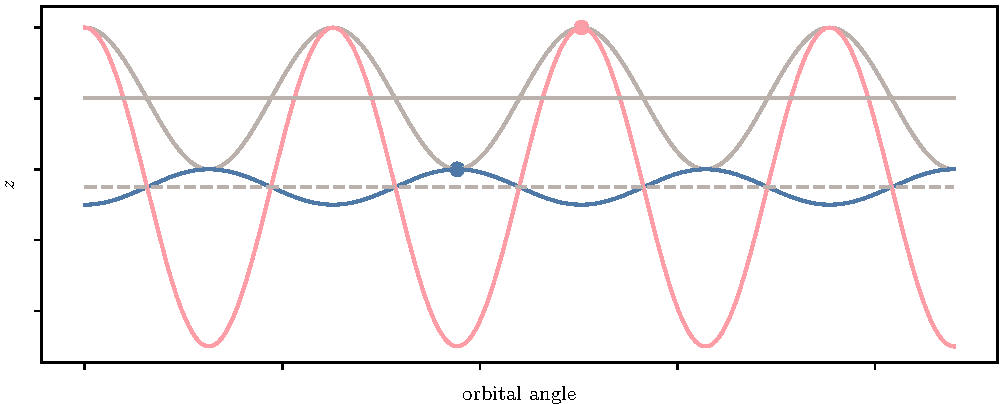
\includegraphics[width=\textwidth]{fig/cartoon.pdf}
\end{center}
\caption{Cartoon approximation showing the effect an error in the
determination of the coordinate midplane can have on orbit integration and
action estimation. The $x$-axis shows the orbital phase and the $y$-axis the
vertical height. The top gray curve depicts an example ``true'' orbit
oscillating about the true midplane (horizontal solid gray line). Consider an
observer who erroneously assumes the midplane is located at the horizontal
dashed line. Suppose this observer measures the phase-space position of the
star at two different orbital phases (teal and orange points). If the
observer were then to integrate the star's orbit using a model potential with
the erroneous midplane, they would obtain the teal and orange curves for the
star's orbit, respectively. The actions estimated from these two  erroneous
orbits would subsequently differ, both from each other and from the actions
estimated for the true orbit (in the potential with the correct midplane).
Hence an incorrect midplane in the potential model assumed will induce
phase-dependence in the actions estimated for a given star in that potential.}
\label{fig:cartoon}
\end{figure*}

In Section~\ref{sec:ref_frame}, we describe the general impact coordinate
system errors have on the measured actions. We then discuss two potential
sources of these coordinate system offsets in
Sections~\ref{sec:mes_err}~and~\ref{sec:local_fire}. In
Section~\ref{sec:mes_err} we discuss the potential errors in measuring the
parameters of the Galactocentric coordinate system. In
Section~\ref{sec:local_fire} we examine the azimuthal variations of the
midplane itself in two sets of simulations: cosmological, hydrodynamical,
zoom-in simulations of Milky Way-mass galaxies from the Feedback in Realistic
Environments (FIRE)
collaboration\footnote{\url{https://fire.northwestern.edu}}
\citep{2014MNRAS.445..581H, 2016ApJ...827L..23W, 2018MNRAS.480..800H}, and a controlled N-body
simulation of a Sagittarius encounter with a galaxy otherwise tailored to the
stellar mass, scale length, and scale height of the Milky Way
\citep{2018MNRAS.481..286L}.

In Section~\ref{sec:discussion}, we discuss the implications of midplane
variations, and the resulting systematic uncertainty in the vertical action,
for action-space analyses. We also estimate the expected midplane variations of the Milky Way based on the observed velocity variations. We
summarize our main results and conclude in Section~\ref{sec:conclusion}.

\section{Motivation} \label{sec:ref_frame}
We first demonstrate the significance  to action computations of a systematic
offset in the determination of the Galactic midplane or distance to the
Galactic center. We will find that such offsets are especially important for
disk-like orbits. The consequences we explore here may also arise from various
other systematic errors. For instance, the axisymmetric Galactic potential
model used in many works to compute actions may not be a good description of
the true potential --- or the parameters used may yield a potential that is
systematically incorrect outside an original fitted region. In this work, we
assume that the Galaxy is perfectly described by our model axisymmetric
potential, and simply explore the consequences of offsets in the determination
of the Galactocentric coordinate system.

\subsection{Effect of Midplane Offset} \label{ssec:cartoon}
We present a cartoon approximation in Figure~\ref{fig:cartoon} to show how an
inaccurate or erroneous determination of the midplane (and hence the
zero-point of the $z$ coordinate) leads to a phase-dependence of the actions
calculated from an orbit specified by a phase-space point and an assumed
potential model. The $y$-axis corresponds to the vertical height of the orbit
and the $x$-axis shows orbital phase. The solid gray curve indicates the
``true'' orbit of the star; that is, its orbit as it oscillates around the
true midplane. The dashed gray line is the midplane location in the potential
model used by an observer to integrate the orbit of the star and hence estimate its actions,
which is offset from the true midplane of the star's orbit. The model
potential is otherwise identical to the one in which the star is actually
moving.

Now suppose this observer makes a measurement of the star's position and
velocity at the teal point or the orange point (i.e. at two different orbital
phases). Then the teal and orange curves correspond to the orbits that the
observer would compute for each point based on the potential model with the
offset midplane. In action space, this would correspond to a different value
of $J_z$ for the teal and orange points. In this way, assuming the wrong
coordinate system induces a phase-dependence in the actions estimated for the
star, which in the correct potential (in this example, the one with the
correct midplane) should be phase-independent.

\subsection{Epicyclic Approximation} \label{ssec:epi_action}

\begin{deluxetable*}{cccccccc}
\tablecaption{Description and names of the three orbits considered in this
work. For the last two columns: $z_{\text{max}}$ is the maximum height of the
orbit while $\frac{1}{2}(R_{\text{max}} - R_{\text{min}})$ is the magnitude of the radial excursions of the orbit. In the epicyclic approximation, $A_z = z_{\text{max}}$ and $A_R = \frac{1}{2}(R_{\text{max}} - R_{\text{min}})$. \label{tab:orbits}}
\tablehead{\colhead{name} & \colhead{initial position} & \colhead{initial
velocity} & \colhead{$J_R$} &
\colhead{$J_{\phi}$} & \colhead{$J_z$} & \colhead{$z_{\text{max}}$} &
\colhead{$\frac{1}{2}(R_{\text{max}} - R_{\text{min}})$}\\ \colhead{ } &
\colhead{$\mathrm{kpc}$} & \colhead{$\mathrm{km}/\mathrm{s}$} &
\colhead{$\mathrm{kpc\,km\,s^{-1}}$} &
\colhead{$\mathrm{kpc\,km\,s^{-1}}$} & \colhead{$\mathrm{kpc\,km\,s^{-1}}$} &
\colhead{$\mathrm{kpc}$} & \colhead{$\mathrm{kpc}$}}
\startdata 
thin-disk & $(8, 0, 0)$ & $(0, -190, 10)$ & 40.3 & -1520 & 0.69 & 0.12 & 1.29 \\
thick-disk & $(8, 0, 0)$ & $(0, -190, 50)$ & 32.5 & -1520 & 23.0 & 0.85 & 1.19 \\ 
halo & $(8, 0, 0)$ & $(0, -190, 190)$ & 32.8 & -1520 & 529.1 & 6.16 & 2.34
\enddata
\end{deluxetable*}

Before turning to numerical methods, we first write down analytically the
systematic error in the actions induced from either a midplane offset or a
Galactocentric radius offset. We use the epicyclic approximation, which
assumes that the motion in the $z$ and $R$ components of the orbit are
decoupled and follow simple harmonic motion about a circular and planar
``guiding orbit'' \citep[][Section~3.2 and references
therein]{2008gady.book.....B}. We refer to the radius of this orbit (the
``guiding radius'') as $R_g$. This approximation is an excellent description
of thin disk-like orbits and a good description of thick disk-like orbits in
an axisymmetric potential (i.e. ignoring the influence of the Galactic bar and
spiral arms). We also make the assumption of a perfectly flat circular
velocity curve with velocity $v_c$, a good approximation near the Solar circle \citep[e.g.][]{2017MNRAS.465...76M}.

Under this approximation, we can write down the cylindrical components
of the orbits as
\beq\label{eq:orbits_epi}
\begin{split}
\phi(t) &= \Omega_c t \\
R(t) &= R_g + A_R \sin{(\kappa t + \alpha)} \\
z(t) &= A_z \sin{(\nu t + \beta)}
\text{,}
\end{split}
\eeq
where $\kappa$ and $\nu$ are the radial and vertical frequencies, $\Omega_c
\equiv v_c/R_g$ is the rotation frequency, $A_z$ and $A_R$ are the amplitudes of
the stellar motion in the vertical and radial coordinates, and $\alpha$ and
$\beta$ are arbitrary constants. Similarly, the velocities of the orbit are
given by:
\beq\label{eq:orbits_vel_epi}
\begin{split}
v_{\phi}(t) &= v_c \\
v_R(t) &= \kappa A_R \cos{(\kappa t + \alpha)} \\
v_z(t) &= \nu A_z \cos{(\nu t + \beta)}
\text{.}
\end{split}
\eeq

In this case, we have that for $J_{\phi}$
\citep[][Section~3.5.3b]{2008gady.book.....B}:
\beq\label{eq:Jphi_epi}
J_{\phi} = R_g v_c\text{,}
\eeq
and for $J_R$ and $J_z$:
\beq\label{eq:JR_Jz_epi}
\begin{split}
J_R &= \frac{E_R}{\kappa} \\
J_z &= \frac{E_z}{\nu} \text{,}
\end{split}
\eeq
where $E_R$ and $E_z$ are the energy per unit mass in the radial and vertical
coordinates, respectively. Therefore,
\beq\label{eq:JR_Jz_epi_energy}
\begin{split}
J_R &= \frac{v_R^2 + \kappa^2 (R-R_g)^2}{2\kappa} \\
J_z &= \frac{v_z^2 + \nu^2 z^2}{2\nu}\text{.}
\end{split}
\eeq
Using Equations~\eqref{eq:orbits_epi} and \eqref{eq:orbits_vel_epi}, we can
simplify this and write
\beq\label{eq:JR_Jz_epi_final}
\begin{split}
J_R &= \frac{\kappa A_R^2}{2} = \frac{v_{R,\text{max}}^2}{2\kappa} \\
J_z &= \frac{\nu A_z^2}{2} = \frac{v_{z,\text{max}}^2}{2\nu}\text{,}
\end{split}
\eeq
where the last equality in each line comes from the fact that $v_{R,\text{max}} = \kappa
A_R$ and $v_{z,\text{max}} = \nu A_z$.

Notice that while the value for each of $J_{\phi}$, $J_R$, and $J_z$ is phase
independent, the contribution from the kinetic and potential terms in
Equation~\eqref{eq:JR_Jz_epi_energy} is phase dependent. Now assume that the
coordinates $(R, z, v_{\phi}, v_R, v_z)$ are offset by $(\Delta R, \Delta z,
\Delta v_{\phi}, \Delta v_R, \Delta v_z)$. We can then apply the standard
propagation of errors formula to Equation~\eqref{eq:JR_Jz_epi_energy}
to determine the error in each of the actions. For $J_{\phi}$, the induced error is:
\beq\label{eq:induced_Jphi}
\frac{\Delta J_{\phi}}{J_{\phi}} = \frac{\Delta R}{R_g} 
                                    + \frac{\Delta v_{\phi}}{v_c}\text{.}
\eeq
For $J_R$, the induced error is:
\beq\label{eq:induced_JR}
\frac{\Delta J_R}{J_R} = \frac{2(R-R_g)}{A_R^2}\Delta R
                         + \frac{2v_R}{v_{R,\text{max}}^2} \Delta v_R \text{.}
\eeq
For $J_z$, the induced error is:
\beq\label{eq:induced_Jz}
\frac{\Delta J_z}{J_z} = \frac{2z}{A_z^2}\Delta z
                         + \frac{2v_z}{v_{z,\text{max}}^2} \Delta v_z \text{.}
\eeq
We have ignored second order contributions.

Since most of the time stars will be at maximum amplitude (i.e. turnaround) in
both $R$ and $z$, we can approximate the order of magnitude of the systematic
error in the actions by
\beq\label{eq:Ji_err_mosttime}
\begin{split}
\frac{\Delta J_{\phi}}{J_{\phi}} &= \frac{\Delta R}{R_g} + \frac{\Delta v_{\phi}}{v_c} \\
\frac{\Delta J_{R}}{J_{R}} &= \frac{2\Delta R}{A_R} \\
\frac{\Delta J_{z}}{J_{z}} &= \frac{2\Delta z}{A_z} \text{,}
\end{split}
\eeq
where we have also ignored second order terms.

In the remainder of this section, we compare our analytic estimates of the
effect of a midplane offset on actions against numerical calculations. A
numerical evaluation of the effect of velocity offsets on actions is deferred
to future work, as we discuss in Section~\ref{ssec:lsr_var}.

\subsection{Numerical Methods} \label{ssec:action_comp}
We now quantify the argument made in Section~\ref{ssec:cartoon} using
numerical computations of the actions for a range of orbits in a model
Galactic potential. We compute actions as in
\citet{2018ApJ...867...31B}, using the code \texttt{gala} v0.3 to perform
orbit integrations and conversion to action space
\citep{2017JOSS....2..388P,Price-Whelan:2018}. To compute actions we use the
torus-mapping technique first presented by \citet{1990MNRAS.244..634M} and
adapted by \citet{2014MNRAS.441.3284S} to calculate actions for an orbital
time-series starting from a phase-space position $(x, v)$ and integrated in a
potential $\Phi$. We use the default \texttt{MWPotential} as our potential,
which is based on the Milky Way potential available in \texttt{galpy}
\citep{2015ApJS..216...29B}. This potential includes a Hernquist bulge and
nucleus \citep{1990ApJ...356..359H}, a Miyamoto--Nagai disk
\citep{1975PASJ...27..533M}, and an NFW halo \citep{1997ApJ...490..493N}, and
is fit to empirically match some observations. We use the Dormand-Prince
8(5,3) integration scheme \citep{Dormand80:integrator} with a timestep of
$1\,\Myr$ and integrate for $5\,\Gyr$, corresponding to $\sim 20$ orbits for a
Sun-like star.

We assume the Sun is located at $(8.2, 0, 0)\,\kpc$. None of our orbit
calculations depend on the value of the LSR in this toy potential (though this
is important when using real data, since the conversion from heliocentric to
Galactocentric coordinates depends on the LSR). In this potential, we have
that the circular velocity $v_{\text{circ}}$ is $231\,\kms$ at the Solar
circle.

Other methods for computing actions are used in the literature. For example,
the St\"ackel Fudge method \citep{2016MNRAS.457.2107S}, which uses a single
St\"ackel potential (with analytic actions) to approximate the Galactic
potential \citep{1985MNRAS.216..273D,2012MNRAS.426.1324B}, was used in many
recent works exploring actions in the Galactic disk
\citep[e.g.][]{2019MNRAS.484.3291T,2018MNRAS.481.4093S,2018arXiv180803278T}.
For disk-like orbits, existing implementations of the St\"ackel Fudge method
are of acceptable accuracy, but since we also consider halo-like orbits in
this work (where the St\"ackel Fudge method is inaccurate) we choose to use
orbit integration and torus mapping throughout \citep{2016MNRAS.457.2107S}.

\subsection{Quantification of the Midplane Effect} \label{ssec:quant}

\begin{figure*}[ht!]
\begin{center}
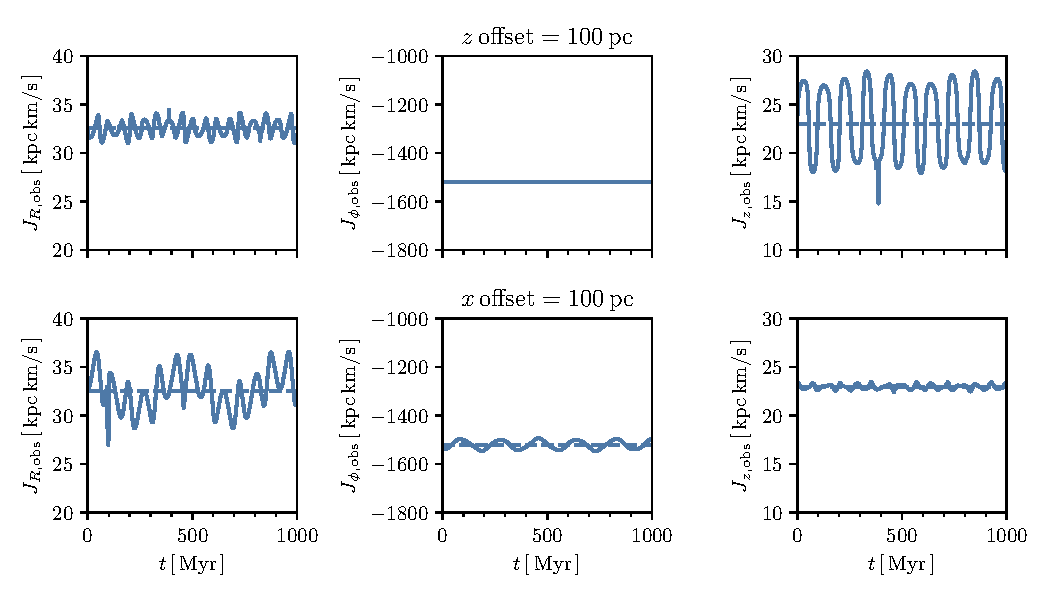
\includegraphics[width=\textwidth]{fig/schmactions_one_orbit.pdf}
\end{center}
\caption{The artificial phase-dependence in the observed actions induced by an
error in the Galactocentric coordinate system. We consider here the thick-disk
orbit, which has actions of $(J_R, J_{\phi}, J_z) = (37.9, -1520,
7.0)\,\actunit$ and $z_{\text{max}}=850\,\pc$ (see Table~\ref{tab:orbits}). We
integrate the orbit according to the procedure laid out in
Section~\ref{ssec:action_comp}, and which we plot in Appendix~\ref{app:orbits}. Then, we subtract $100\,\pc$ from the $z$
value (upper panels) or the $x$ value (lower panels) of each
position in the orbit, corresponding to an erroneous observer assuming a
midplane (upper) or solar radius (lower) that is off by
$100\,\pc$. We then allow an immortal observer to observe the orbit over
$1\,\Gyr$ and perform the same orbit integration procedure at each timestep,
and report the values of the actions. The computation of $J_{\phi}$ is
pristine to errors in $z$, with only numerical artifacts remaining. Only small
errors are induced in $J_R$, with the middle $90\%$ of values over the $\Gyr$
being within $\sim8\%$ of the true $J_R$. As expected, large errors are
induced in $J_z$ with a $100\,\pc$ offset in $z$, with the middle $90\%$ of
values being within $\sim43\%$ of the true $J_z$. The $x$ offset induces
uncertainties in $J_R$, $J_{\phi}$, and $J_z$ of $\sim21\%$, $\sim3\%$, and $\sim3\%$.}
\label{fig:one_orbit_wrong_ref}
\end{figure*}

\begin{figure}
\begin{center}
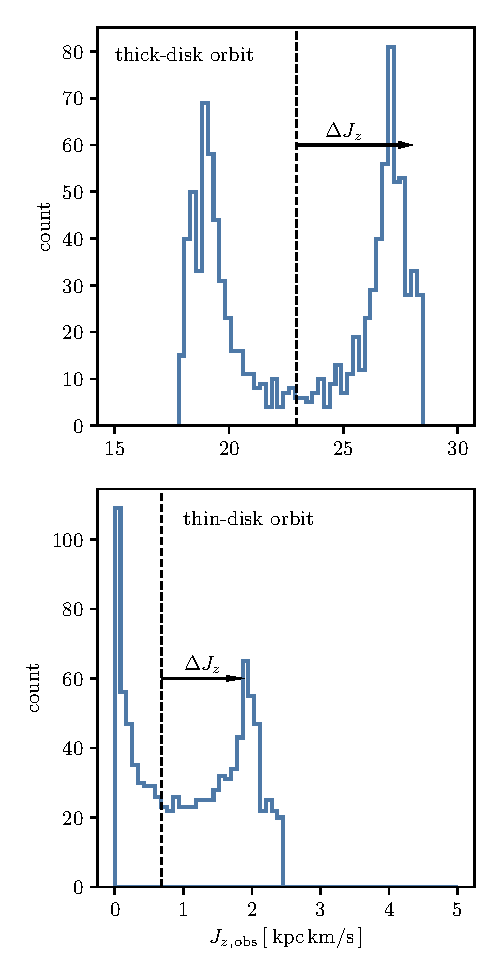
\includegraphics[width=\columnwidth]{fig/schmactions_Jz_zerr_hist.pdf}
\end{center}
\caption{A histogram of the observed values in $J_z$ for the thick-disk (top panel) and thin-disk (bottom panel) orbits
assuming a $z$ offset of $100\,\pc$. One can see that if the observed $z$
values have a bias (from e.g. an incorrectly computed midplane), then the
induced error distribution in $J_z$ is decidedly non-Gaussian. Therefore, any
sort of error propagation must take this into account. Intuition for the shape
of each panel is given in the text. We also plot one half the 95\uth{}
percentile minus the 5\uth{} percentile of each distribution as a horizontal
arrow anchored on the true $J_z$ value. We call this $\Delta J_z$ and will use
it (along with the similarly defined $\Delta J_R$ and $\Delta J_{\phi}$) to
empirically describe the error distribution. We see that $\Delta J_z$ roughly
corresponds to the distance from the true $J_z$ value to one of the modes of
the distribution of observed $J_z$ values.}
\label{fig:Jz_hist}
\end{figure}

We quantify how a systematic error in the Galactocentric coordinate system
induces phase-dependence in the \emph{observed} actions. We will consider three
orbits in the model potential described in Section~\ref{ssec:action_comp} that
are typical of stars in the stellar thin disk, stellar thick disk, and the
stellar halo. We summarize their initial positions in phase space and the
actions computed by integrating their orbits in the correct potential in
Table~\ref{tab:orbits}. Each orbit, integrated without systematic coordinate
errors, is plotted in Appendix~\ref{app:orbits}. We will refer to these orbits
by their names (thin-disk, thick-disk, halo) henceforth.

We begin with the thick-disk orbit. Consider an immortal observer who
can measure the thick-disk star's phase-space position at many different times
(and hence different orbital phases). However, the immortal observer uses a coordinate system in which
the midplane is systematically offset in height by $100\,\pc$ from its actual
location --- i.e. we subtract the vector $(0, 0, 100)\,\pc$ from each position
in the orbit. This corresponds to the immortal observer physically located at
e.g. the position $(8, 0, 0)\,\kpc$ in the coordinate system of the true
potential, but erroneously thinking they are located at $(8, 0, 0.1)\,\kpc$.

We consider that the immortal observer makes a measurement every $\Myr$. At each measurement, we compute the actions as outlined above using the true potential but by specifiying the star's starting position using the systematically offset coordinate system.
Essentially we are shifting the
integrated orbit and then reintegrating at each point along the shifted orbit,
where the shifted orbit is the observed orbit. The erroneous computed actions
for each phase-space starting point are shown for the first $\Gyr$ of the
orbit in the upper panels
Figure~\ref{fig:one_orbit_wrong_ref}.\footnote{Occasionally the numerical
scheme fails and very large actions are reported by \texttt{gala}---we perform
a $5\sigma$ clip on each action to exclude such orbits, but this only excludes
a total of $5$ orbits out of the $1000$ considered for
Figure~\ref{fig:one_orbit_wrong_ref}. Some numerical artifacts remain, but the
vast majority of orbits are computed properly.}
    
We also perform the same procedure but assume a $100\,\pc$ offset in the $x$
component (i.e. subtracting the vector $(100, 0, 0)\,\pc$) in the lower
panels. This is equivalent to a systematic offset in the determination of the
distance from the Sun to the Galactic center.

Figure~\ref{fig:one_orbit_wrong_ref} shows that the actions computed in the
offset coordinate systems depend on the time (i.e. orbital phase) at which the
star's phase-space position is observed. To the immortal observer this would
appear as time-dependence in the actions, which appear to oscillate around
their value using the correct coordinate system even though in this example
the observer is using the correctly constructed best-fit static, axisymmetric
potential. The relative size of the phase variation in each action depends on
the direction of the systematic offset as well as the true values of the
actions (i.e. the type of orbit). In reality we will have one measurement of
the phase-space position to work with, in which case the determination of the
orbital phase in $R$ or $z$ is degenerate with the degree of systematic offset
in that coordinate (see Figure~\ref{fig:cartoon}).  In the following we
therefore quote percentile ranges for the possible values computed for each
action as a proxy for the effect of these systematic errors in the coordinate
system.

For a systematic offset in $z$ (upper panels), the
95\textsuperscript{th} minus 5\textsuperscript{th} percentiles are $2.2$ and
$6.2\,\actunit$ for $J_R$ and $J_z$, respectively. These are fractional errors
of $5.7\,\%$ and $86\,\%$, respectively. The error induced in $J_{\phi}$ is
negligible, as expected since $J_{\phi}$ only depends on the $x$- and
$y$-components of the position and velocity of the stars.\footnote{In practice,
however, $J_{\phi}$ is computed as part of the torus-fitting method.} It is worth
pointing out that a $100\,\pc$ error in an orbit with
$z_{\text{max}}=850\,\pc$ --- a $12\%$ error
--- induced an $86\%$ error in the computation of $J_z$.

For a systematic offset in $x$ (or distance to the Galactic center), the
95\textsuperscript{th} minus 5\textsuperscript{th} percentiles are $6.9$,
$47$, and $0.71\,\actunit$ for $J_R$, $J_{\phi}$ and $J_z$, respectively.
These are fractional errors of $21\%$, $3.1\%$ and $3.1\%$, respectively ---
despite only a $1.2\%$ error in the distance to the Galactic center.

In Figure~\ref{fig:Jz_hist} we plot a histogram of the observed values of
$J_z$ for the thick-disk orbit (top panel) and thin-disk orbit (bottom panel) assuming a $z$ offset of $100\,\pc$ (i.e. as in the upper
right panel of Figure~\ref{fig:one_orbit_wrong_ref}). The true value of $J_z$
is plotted as a vertical dashed line. Here we see that the errors in $J_z$
induced by a systematic offset in $z$ are non-Gaussian and bimodal.
Furthermore, neither of the modes lie at zero. In other words, neither of the
modes of the distribution of observed $J_z$ values are centered on the true
$J_z$ (i.e. the $J_z$ computed with no offset in $z$). In the case of the
thin-disk orbit (bottom panel), we see that, in addition to the prior
complications, the error distribution is not even centered on null. This comes
about when the midplane error is $\gtrsim z_{\text{max}}$, where
$z_{\text{max}}$ is the maximum height of the orbit, equivalent to $A_z$ in the epicyclic approximation (see
Section~\ref{ssec:epi_action}).

\begin{figure*}[htb!]
\begin{center}
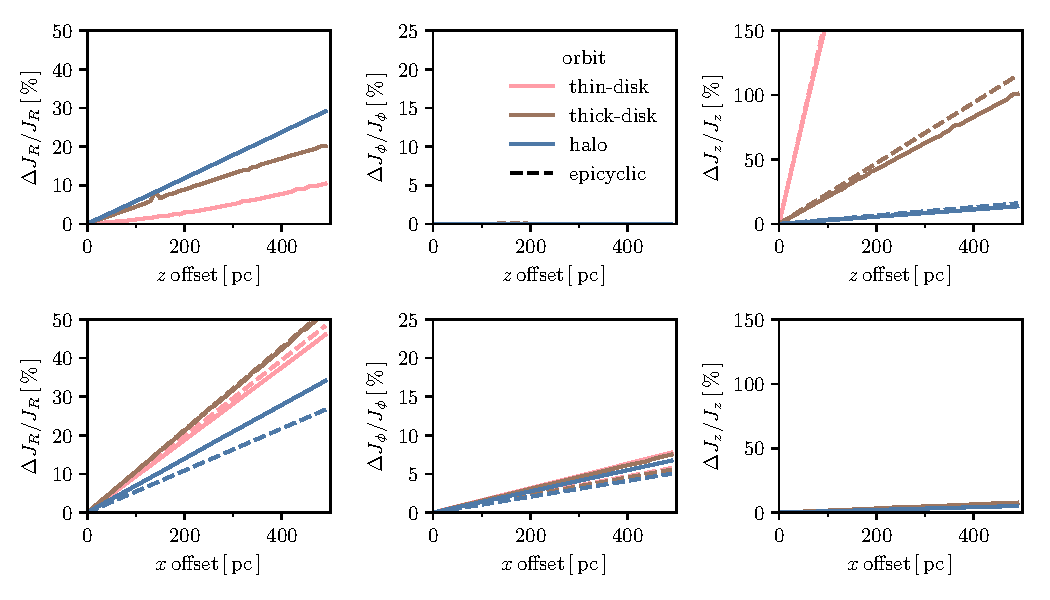
\includegraphics[width=\textwidth]{fig/schmactions_many_orbits.pdf}
\end{center}
\caption{We report one half the 95\uth{} minus 5\uth{} percentile of the error
in the measured action ($\Delta J_i$) from coordinate system errors for the
thin, thick, and halo orbits (Table~\ref{tab:orbits}). See discussion in the
text for the justification in using this to measure the magnitude of the
induced error. The left, center, and right panels show the
result for $J_R$, $J_{\phi}$, and $J_z$, respectively. The upper panels
consider an offset in $z$ and the lower panels consider an offset in $x$
(equivalently, an offset in the Solar radius). In some panels we also plot as
dashed lines the epicyclic prediction of the induced action error
(Equation~\eqref{eq:Ji_err_mosttime}). In the epicyclic approximation, a $z$
offset only induces an error in $J_z$ --- for all three orbits the epicyclic
approximation is a good description of the $J_z$ error. An $x$ offset induces
an error in $J_R$ and $J_{\phi}$. The error in $J_R$ is somewhat
well-described for the thin-disk and thick-disk orbits, and a poor description
for the halo orbit. For $J_{\phi}$, the epicyclic approximation is not a good
description for any orbit.}
\label{fig:many_orbit_wrong_ref}
\end{figure*}

We now describe the intuition behind the shape of Figure~\ref{fig:Jz_hist}.
Consider first the thick-disk orbit (top panel), where the offset in $z$
is much less than $z_{\text{max}}$ of the orbit. The peaks in the distribution
correspond to the turning points of the orbit (or points of maximum vertical
amplitude), where $v_z \sim 0$ and where the star is on most of it orbit.
This is why the distribution is peaked on these values. For the thin-disk
orbit (bottom panel), the offset in $z$ is comparable to
$z_{\text{max}}$. Now, there will be some points in the orbit where $v_z = 0$
and $z=0$ (in the observed, erroneous coordinate system). At these points, the
computed $J_z$ will vanish. The asymmetry and systematic offset then comes
about because of the constraint that $J_z \geq 0$.\footnote{This is similar to
arguments in cosmology for why gravity produces non-Gaussianity in the density
field, since the density cannot become negative but it can grow arbitrarily
large.}

Empirically describing the error distribution shown in
Figure~\ref{fig:Jz_hist} is difficult. Of course, Gaussian summary statistics
are not adequate. We therefore elect to measure this error by computing one
half the 95\uth{} percentile minus the 5\uth{} percentile of the distribution
of observed action values. We refer to this quantity as $\Delta J_i$ for each
action value. We plot this quantity in Figure~\ref{fig:Jz_hist} as a
horizontal arrow anchored on the true action value. Because of the bimodality
of the error distribution, this quantity roughly measures the distance from
the true action value to the peak of one of the modes. Furthermore, this
bimodality also implies that $\Delta J_i$ is not very sensitive to the exact
percentiles used. This summary statistic does not reflect the bias induced
when the midplane error is $\gtrsim z_{\text{max}}$.

We now repeat the same procedure as in Figure~\ref{fig:one_orbit_wrong_ref}
but for systematic offsets between $0$ and $500\,\pc$ in the $z$ and $x$
components. In Figure~\ref{fig:many_orbit_wrong_ref}, we report one half the
95\uth{} minus 5\uth{} percentile divided by the true action value ($\Delta
J_i/J_i$) for the three different fiducial orbits in Table~\ref{tab:orbits}.
The thick-disk (\thickcolor) orbit is the one from
Figure~\ref{fig:one_orbit_wrong_ref}, but we also now consider the effect on
the action determined for the thin-disk (\thincolor) and halo (\halocolor)
orbits.

The upper row of Figure~\ref{fig:many_orbit_wrong_ref} shows the spread induced
in each action for an offset in the $z$-component (i.e. the Galactic
midplane). In the lower row we consider offsets in the $x$ component
(i.e. the Solar radius). The left, center, and right columns
show the fractional spread in the values computed for $J_z$, $J_{\phi}$, and
$J_R$, respectively. We compute the fractional spread $\Delta J_i/J_i$, where
$\Delta J_i$ is defined in the previous paragraph and $J_i$ is the action
value computed in the true coordinate system, over the course of the first
$\Gyr$.

In the upper middle panel of Figure~\ref{fig:many_orbit_wrong_ref},
there is essentially no spread in the determination of $J_{\phi}$. This is
expected since $J_{\phi}$ is independent of $z$ and is
thus unaffected by offsets in $z$, as discussed earlier. Indeed, the result we found in
Figure~\ref{fig:one_orbit_wrong_ref} for the thick-disk orbit holds for all
orbit types. This is also a demonstration of the robustness of the orbit
integration and action calculation methods we use.
 
The upper right panel of Figure~\ref{fig:many_orbit_wrong_ref} shows
that the fractional error in $J_z$ is more exaggerated for more planar
(disk-like) orbits. For the thin-disk orbit, a systematic offset of
$\sim15\,\pc$ in the $z$ coordinate already results in $25\%$ deviations in
the actions. The required offset for $25\%$ deviation is $\sim120\,\pc$ for
the thick-disk orbit. The halo orbit is relatively resistant to errors in the
midplane, with only $\sim15\%$ error in $J_z$ out to a midplane offset of
$500\,\pc$.

For the offset in the Solar radius (lower panels), the error is largest
for $J_R$, with some deviations resulting in $J_{\phi}$ and relatively small
deviations in $J_z$. In the lower middle and lower right panels
all three lines nearly overlap.

In each panel of Figure~\ref{fig:many_orbit_wrong_ref}, where relevant, we
include the estimation of the action errors derived under the epicyclic
approximation from Equation~\eqref{eq:Ji_err_mosttime}, with $\Delta v_{\phi}=0$, as dashed lines in the color of each orbit. This equation is
relevant since during most of the orbit the star will be at maximum radial and
vertical amplitude and we do not consider velocity offsets. Note that we
consider an error in the $x$-coordinate $\Delta x$, which is not exactly the
same as $\Delta R$. For observations of stars close to us, we have that
$\Delta x \sim \Delta R$, but for the experiment performed in this Section we
consider observations of the star throughout its entire orbit. This introduces
a factor of $2/\pi$ when converting from $\Delta x$ to $\Delta R$, which we
derive in Appendix~\ref{app:deltax}.

The epicyclic approximation is a good predictor of $\Delta J_z$, even for halo
orbits. It performs similarly for $\Delta J_R$, now underpredicting for halo orbits
and slightly overpredicting for thin-disk orbits. Note that for the particular
orbits we chose, the thin-disk orbit has slightly larger $A_R$ than the
thick-disk orbit, and so we expect the epicyclic approximation to perform
slightly worse. The epicyclic approximation underpredicts $\Delta J_{\phi}$ for all
orbits.

\begin{figure}
\begin{center}
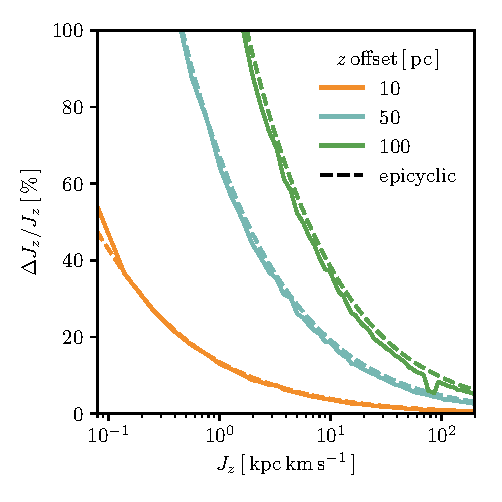
\includegraphics[width=\columnwidth]{fig/schmactions_many_orbits_Jz_fun.pdf}
\end{center}
\caption{The fractional error in $J_z$ as a function of $J_z$ for a few
different offsets in $z$. All orbits have the same initial position of $(8, 0, 0)\,\kpc$ and velocity $(-190, 0, v_z)\,\kms$, where we vary $v_z$. We show this for a $z$ offset of $10, 50, 100\,\pc$
(orange, teal, and green respectively). As before, the error ($\Delta J_z$) is
one half the 95\uth{} minus 5\uth{} percentile of the distribution of observed
$J_z$ values over the course of the orbit. There are large errors for
thin-disk like orbits ($J_z \sim 0.5\,\actunit$), even for a small midplane
offset of $10\,\pc$. As dashed lines in each color we also plot the prediction
for $\Delta J_z/J_z$ from the epicyclic approximation
(Equation~\eqref{eq:Ji_err_mosttime}), which shows excellent agreement with
the numerically computed values.}
\label{fig:dJz_fun_Jz}
\end{figure}

To further understand the effect of the midplane error, we also plot the
fractional error in $J_z$ as a function of $J_z$ for $z$ offsets of $10, 50,
100\,\pc$ (orange, teal, and green, respectively) in
Figure~\ref{fig:dJz_fun_Jz}. For each orbit, we set the initial position to be $(8,0,0)\,\kpc$ and the initial velocity to be $(-190, 0, v_z)\,\kms$, where we vary $v_z$. For a thin disk-like orbit
($J_z\sim0.5\,\actunit$), even a $10\,\pc$ offset in $z$ is enough to induce a
$\sim25\%$ error in $J_z$. For larger values of $J_z$, the fractional errors
are suppressed, but the induced error can still be large depending on how
great the $z$ offset is. We also plot the epicylic prediction for $\Delta J_z
/ J_z$ from Equation~\eqref{eq:Ji_err_mosttime} as dashed lines for each $z$
offset. We find that the epicyclic approximation matches the numerical
estimate quite well.

\section{Coordinate System Offsets I. Measurement Errors} \label{sec:mes_err}
We consider the first potential source of coordinate system offsets which
would generate the action errors described in Section~\ref{sec:ref_frame}:
uncertainties in measurements of the position and velocity of the Sun relative
to the Galactic center. Converting from heliocentric to Galactocentric
coordinates relies on these measurements. Therefore, errors in their values
will induce a systematic offset in the Galactocentric phase-space position of
any observed star.

\subsection{Galactic Center}
First, one must define the center of the Galaxy. This is usually taken to be
the location of the central supermassive black hole, Sagittarius~A\textsuperscript{*}
\citep[\sgra{}, e.g.][]{2004ApJ...616..872R}. From stellar motions near
\sgra{}, the distance from the Sun to
\sgra{}, referred to as $R_0$, can be precisely measured \citep{2009ApJ...692.1075G,
2018AA...615L..15G}, with a recent measurement using near-infrared
interferometry of $8.178 \pm 0.035$~kpc \citep{2019arXiv190405721A}.

\subsection{Galactic Orientation}
Second, one must define the angular orientation of the Galaxy. This was
defined in 1958 by the IAU subcomission 33b \citep{1960MNRAS.121..123B} by
defining the coordinates of the Galactic center in B1950 coordinates as
(17:42:26.6, -28:55:00) and the North Galactic pole as (12:49:00, +27:24:00).
These two quantities, together with $R_0$, define the orientation of the
Galactic plane. However, there is growing evidence that the stellar midplane
is tilted relative to this coordinate system \citep{2014ApJ...797...53G,
2016ARAA..54..529B}, though not the H~\textsc{ii} midplane
\citep{2019ApJ...871..145A}.

\subsection{Solar Height}
Third, one must define the Sun's vertical distance from the Galactic midplane,
which can be determined by identifying where the stellar density and
velocities reach a maximum (effectively the median height of all disk stars).
The Solar height is usually taken to be $\sim 25\,\pc$
\citep{2001ApJ...553..184C}, with a more recent measurement from \textit{Gaia}
DR2 placing it at $20.8 \pm 0.3\,\pc$ \citep{2019MNRAS.482.1417B}. Another
strategy is to use the cold gas or H~\textsc{ii} regions in the disk to define
the Galactic midplane, leading to slightly different values (by $\sim 5\,\pc$)
for the Sun's relative height \citep[e.g.][]{2019ApJ...871..145A}. A pre-{\em
Gaia} review of these measurements is given by \citet{2016ARAA..54..529B}.

\subsection{Local Standard of Rest}
Finally, one must define the LSR, or mean velocity of
stars near the Sun relative to the Galactic center (which is defined to have
zero velocity), and the velocity of the Sun relative to the LSR. The radial
($U_{\odot}$) and vertical ($W_{\odot}$) components are computed by taking the
mean motions of different stellar groups \citep[e.g.][]{2012MNRAS.427..274S}.
The azimuthal component ($V_{\odot}$) is more difficult to measure, but can be
modeled using the asymmetric drift relation \citep{2008gady.book.....B}. The
values of the components of the LSR are usually taken from
\citet{2010MNRAS.403.1829S}. The value of the circular velocity is taken to be
$\sim 220\kms$ \citep[e.g.][]{2012ApJ...759..131B}.

\vspace{6pt}

Considerable effort has been placed on each of these measurements, but
uncertainties remain, and detailed dynamical modeling across the disk ---
particularly for dynamically cold stars --- may have to take them into
account. For instance, the discrepancy of $\sim 5\,\pc$ between the midplane
defined by stars and by gas will induce a $\sim10\%$ error in $J_z$ for an
orbit with $z_{\text{max}}\sim100\,\pc$ (see Section~\ref{sec:ref_frame}).

\section{Coordinate System Offsets II. Azimuthal Midplane Variations in
Simulations}
\label{sec:local_fire}

We now consider a second source of systematic offsets in the Galactocentric
coordinate system: intrinsic variations of the midplane across the disk. In
this work we specifically consider azimuthal variations in the midplane as
defined by the stellar mass density. We use two sets of simulations of Milky
Way-mass galaxies to estimate the size of this effect.

\subsection{Description of FIRE Simulations} \label{ssec:cosmozoom}
The FIRE cosmological hydrodynamic simulations
\citep{2014MNRAS.445..581H,2018MNRAS.480..800H} use the zoom-in technique
\citep[e.g.][]{1993ApJ...412..455K,2014MNRAS.437.1894O} to model the formation
of a small group of galaxies at high resolution in a full cosmological
context.  Feedback from supernovae, stellar winds, and radiation from massive
stars is implemented at the scale of star forming regions following stellar
population synthesis models, generating galactic winds self-consistently
\citep{2015MNRAS.454.2691M, 2017MNRAS.470.4698A} while reproducing many
observed galaxy properties, including stellar masses, star formation
histories, metallicities, and morphologies and kinematics of thin and thick
disks \citep{2014MNRAS.445..581H, 2016MNRAS.456.2140M, 2017MNRAS.467.2430M,
2016ApJ...827L..23W, 2018MNRAS.481.4133G, 2018MNRAS.480..800H}. For this work,
we focus on the three Milky Way-mass zoom-ins considered in
\citet{2018arXiv180610564S}, which were simulated as part of the
\textit{Latte} suite and show broad agreement of many of their global
properties with observations of the Milky Way \citep{2016ApJ...827L..23W,
2018MNRAS.481.4133G}. The $\z = 0$ snapshots\footnote{In this work, to avoid
confusion with the vertical height $z$, we refer to cosmological redshift as
$\z$.} of these three simulations, named \mi{}, \mf{}, and \mm{} for
shorthand, are publicly available alongside associated mock \textit{Gaia} DR2
catalogues generated from them.\footnote{\url{http://ananke.hub.yt}}

\begin{deluxetable*}{cccccc}[htb!]
\tablecaption{Stellar and gas disk scale heights of the real Milky Way and the
simulated galaxies considered in this work. For comparison, we also give the softening lengths for the simulated galaxies.\label{tab:scale_height}}
\tablehead{\colhead{galaxy} & \colhead{cold\tablenotemark{a} gas disk} &
\colhead{stellar thin disk} & \colhead{stellar thick disk} & \colhead{cold gas
softening length} & \colhead{stellar softening length} \\
\colhead{} & \colhead{(pc)} & \colhead{(pc)} & \colhead{(pc)} & \colhead{(pc)}
& \colhead{(pc)} }
\startdata
Milky Way\tablenotemark{b} & 40 & 300 & 900 & \nodata & \nodata \\
\mi\tablenotemark{c} & 800\tablenotemark{d} & 480 & 2000 & 12.4 & 11.2 \\
\mf\tablenotemark{c} & 360 & 440 & 1280 & 12.5 & 11.2 \\
\mm\tablenotemark{c} & 250 & 290 & 1030 &10.3 & 11.2 \\
\enddata
% \tablerefs{\citet{2016ARAA..54..529B,2018arXiv180610564S,2008ApJ...673..864J}}
\tablenotetext{a}{$T<1000$ K}
\tablenotetext{b}{\citet{2008ApJ...673..864J,2016ARAA..54..529B}}
\tablenotetext{c}{\citet{2018arXiv180610564S}}
\tablenotetext{d}{The azimuthally averaged gas vertical density profile in
\mi{} is nearly constant to this height, though individual regions show smaller
scale heights and dense clouds.}
\end{deluxetable*}

These simulations contain dark matter particles of mass $\sim35,000\,\Msun$,
gas particles of mass $\sim 7000$ to $20,000\,\Msun$, and star particles
of mass $\sim 5000 \text{--} 7000\,
\Msun$, with the lower end
coming from stellar evolution \citep{2018arXiv180610564S}. Softening lengths
for dark matter and star particles are fixed at $112\,\pc$ and $11.2\,\pc$,
respectively.\footnote{This is $2.8$ times the often-quoted
Plummer-equivalent.} The gas softening length is adaptive, but at $\z=0$ the
median softening length for cold ($T < 10^4\,\text{K}$) gas particles around
roughly solar positions (with galactocentric cylindrical radii within $0.5\,\kpc$ of
$8.2\,\kpc$ and $\abs{z}<1\,\kpc$) is $12.4$, $12.5$, and $10.3\,\pc$ for \mi{},
\mf{}, and \mm{}, respectively. These values are summarized in
Table~\ref{tab:scale_height}, along with measurements of the stellar and gas
disk scale heights.

The softening lengths used in the simulations can affect the ability to
resolve the very thinnest planar structures, which in turn can affect how much
the density-based midplane varies as a function of azimuth. The Milky Way's
dense, star-forming gas disk is thought to have a scale height of about
$40\,\pc$, $\sim3\textup{--}4$ times the cold gas softening length
\citep{2019ApJ...871..145A}. The thin stellar disk has a scale height of
about $300\,\pc$, $\sim30$ times the stellar softening length
\citep{2008ApJ...673..864J}. We therefore expect that resolution effects
may still be affecting the scale heights of these components in the
simulations, especially the cold gas. Indeed, the stellar scale heights of the
simulated galaxies are equal to or larger than the Milky Way's while the gas scale
heights are significantly larger (although the proper basis comparison is less
clear in the case of the gas; the quoted value for the Milky Way comes from
studies of high-mass star-forming regions). As noted above, the midplanes
defined by gas and stars can be tilted with respect to one another as well,
precluding extending the precision of the gas midplane definition to the
stellar component.

Cosmological simulations of Milky Way-mass galaxies are not perfect
representations of the true Milky Way in other ways as well,\footnote{The failure of cosmological simulations to exactly reproduce the Milky Way is not entirely due to limitations of the numerical model. Candidate Milky Way-like galaxies are chosen solely on their mass and isolation, for which there are a wide variety of possible galaxies with qualitatively different properties.} as discussed in
\citet{2018arXiv180610564S}. For instance, the velocity structure of \mi{} is
closer to M31's than the Milky Way's (Loebman et al. in prep). However, in
this work we are most interested in the global properties of the potential,
and specifically in deviations from axisymmetry. From this perspective, the
simulated galaxies are actually \emph{more} axisymmetric than we might expect
of the Milky Way. While they have prominent spiral arms, none has as strong a
bar as the Milky Way does at present day, and none has a nearby companion like the
Large Magellanic Cloud. One of the three we consider (\mf) does have an
ongoing interaction with a satellite galaxy similar to Sagittarius, which has
punched through the galactic disk outside the solar circle and induced some
warping.

In this work, we take the galactocentric coordinate system described in
Section 3 of \citet{2018arXiv180610564S} as our fiducial coordinate system for
each galaxy. In short, the center of the galaxy is found iteratively. The
center of mass velocity is then determined by all star particles within
$15\,\kpc$ of this center. The galaxy is then rotated onto a
principal axis frame determined by stars younger than $1\,\Gyr$ inside of the
fiducial solar radius $R_{0} = 8.2\,\kpc$, such that the disk plane is the
$x$--$y$ plane.

\subsection{Description of Milky Way-Sagittarius Interaction Simulation} 
\label{ssec:sag_sim}
In addition to the cosmological zoom-ins, we will also briefly consider results
from a toy Sagittarius encounter simulation. This simulation offers us the
ability to see how the midplane varies in a more controlled environment. The
details of the simulation are given in \citet{2018MNRAS.481..286L}, but we
briefly summarize the most relevant details here. For the Milky Way, the dark
halo is modeled as a Hernquist sphere of mass $10^{12}\,\Msun$ and scale
length of $52\,\kpc$, the disk modeled as an exponential disk with a scale
radius of $3.5\,\kpc$, scale height $0.53\,\kpc$, and mass
$6\times10^{10}\,\Msun$, a Hernquist bulge of mass $10^{10}\,\Msun$ and scale
length $0.7\,\kpc$ \citep{1990ApJ...356..359H}. Sagittarius is modeled as a
dark matter Hernquist sphere of mass \Gus{something} and scale length
\Gus{something}, along with a stellar component modeled as a Hernquist sphere
of mass $6.4\times10^8\,\Msun$ and scale radius $0.85\,\kpc$. All components
are realized with live distributions of N-body particles; the Milky Way and Sagittarius are
each initialized to be in equilibrium in isolation \Gus{check!}.

The mass resolution of the simulation is $2.6\times10^4$, $1.2\times10^4$, and
$1.0\times10^4\,\Msun$ for the dark matter, disk, and bulge components, respectively.
For the disk and bulge components, a softening length of $30\,\pc$ is used
whereas for the halo a softening length of $60\,\pc$ is used. For Sagittarius,
the softening length for the dark matter and the stars is $60$ and $40\,\pc$,
respectively.

The fiducial coordinate system for these toy simulations is the rest frame of
the aligned toy galaxy at the beginning of the simulation.

\subsection{The Local Midplane} \label{ssec:local_midplane}
Using the two sets of simulations, we determine the local midplane that an
observer might measure if they were situated in each of these galaxies as a
function of azimuth at the solar circle. Starting from the coordinate system
described in the previous section, which is approximately aligned so that the
$z$-coordinate is perpendicular to the disk plane, we place our imaginary
observer at $z=0$ and a galactocentric cylindrical radius of $8.2\,\kpc$ and vary the azimuth
between $0<\phi<2\pi$.\footnote{The immortal observer also has warp drive, allowing them to travel around the galaxy much more quickly than its dynamical timescale.} At
each value of $\phi$ we then compute the median $z$ for stars within a
cylinder of radius $0.5\,\kpc$ and height $1\,\kpc$ perpendicular to the
fiducial disk. We then re-define the new midplane of the cylinder to be the
median $z$, re-select stars, and iterate until the median $z$ value converges.
We find that only $10$ iterations of this procedure are necessary for
convergence. The resulting median $z$ is taken to be what our observer would
measure as the local Galactic midplane at each $\phi$.

\begin{figure*}[htb!]
\begin{center}
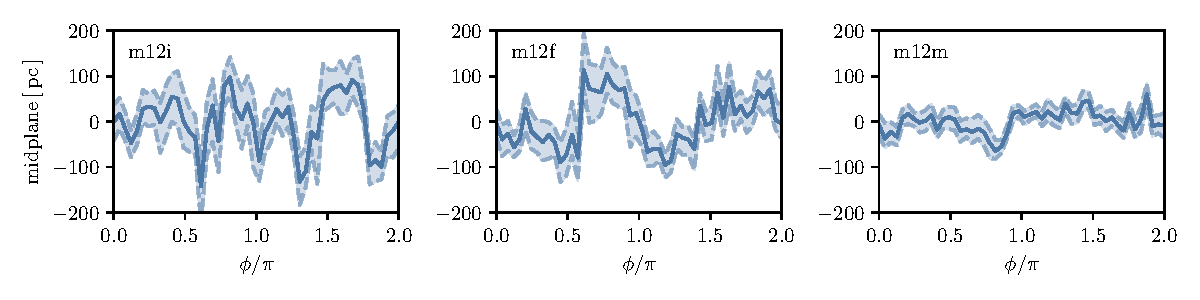
\includegraphics[width=\textwidth]{fig/midplane_fit.pdf}
\end{center}
\caption{The local midplane determined at the fiducial Solar radius
($8.2\,\kpc$) for the three FIRE galaxies \mi{}, \mf{}, and \mm{} (left,
center, and right panels) as a function of azimuthal angle. All calculations are done at
cosmological redshift $\z =0$. The local midplane is determined at a position
$\phi$ by taking the median height of all stars within $R=0.5\,\kpc$ and
$z=1\,\kpc$ (in cylindrical coordinates). The procedure is performed again
using the new height $10$ times to converge on the local midplane height. In
order to allow for the possibility that the fiducial galactocentric coordinate
system is incorrect, we subtract the best fit $A\sin{(\phi+B)}+C$ curve from
each panel --- this figure is reproduced with the original midplane
determination (i.e. before subtracting the best fit sine curve) in
Appendix~\ref{app:lsr}. We then bootstrap resample $1000$ times on all stars
within a $2\,\kpc$ height of the fiducial midplane to determine $1\,\sigma $
error bars, which we report as dashed lines.}
\label{fig:midplane}
\end{figure*}

\begin{figure*}[htb!]
\begin{center}
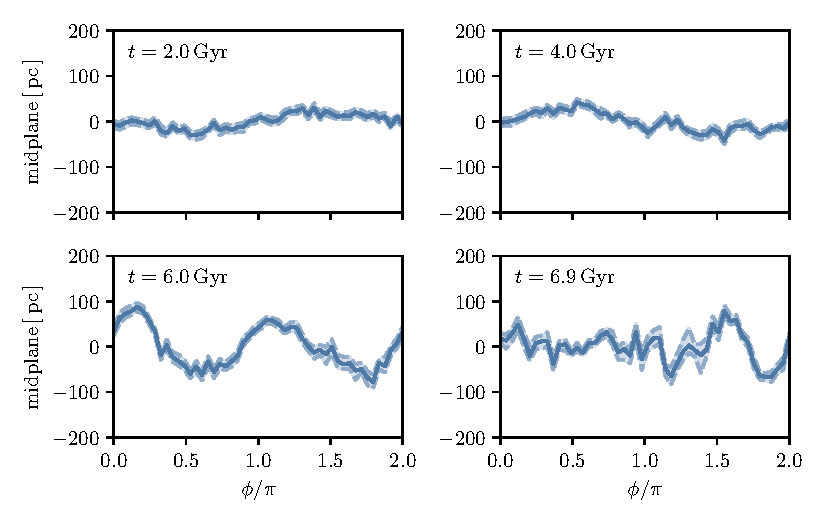
\includegraphics[width=342.078286667pt]{fig/midplane_fit_chervinsim.pdf}
\end{center}
\caption{The local midplane determined at the fiducial Solar radius
($8.2\,\kpc$) for 4 different time steps from toy simulations
of a Sagittarius encounter with the Milky Way \citep{2018MNRAS.481..286L}. As
before, we have subtracted the best fit $A\sin{(\phi+B)}+C$ curve to account
for inaccuracies in the galactocentric coordinate system. Error bars are
calculated as in Figure~\ref{fig:midplane}. (\Gus{Check:}) The upper
panels show the midplane as a function of azimuth before the first encounter
near the Solar circle at $t=2.0\,\Gyr$ and $t=4.0\,\Gyr$. As later encounters occur which bring the
Sagittarius-like object closer to the Solar circle, we can see that stronger
midplane variations result. In fact, one can see that an $m=2$ mode is excited
in the lower left panel at $t=6.0\,\Gyr$ --- this is consistent with Figure~17 of
\citet{2018MNRAS.481..286L}, which shows that an $m=2$ mode is excited (note
that $m=0$ and $m=1$ modes are stronger, but these are removed in our
sine-curve subtraction). The fact that the $t=6.9\,\Gyr$ panel looks
qualitatively similar to the panels from the FIRE simulations
(Figure~\ref{fig:midplane}) is evidence that the midplane variations are
produced in part by mergers.}
\label{fig:midplane_chervin}
\end{figure*}

This procedure assumes perfect density estimation, and therefore perfect
corrections for extinction within the cylinder defining the ``solar
neighborhood.'' Imperfect extinction correction is likely to increase the
amplitude of the estimated fluctuations in $z$.

To account for the effect of particle noise, we bootstrap resample
stars within a cylinder of stars with height $2\,\kpc$ and the same radius
$1000$ times and determine the $1\,\sigma$ error bars by repeating the
midplane determination with those reselection of stars.

To allow for potential small inaccuracies in the determination of the original
fiducial coordinate system, we also subtract the best fit $\text{A}
\sin{\left(\phi + \text{B}\right)} + \text{C}$ curve from the midplane as a
function of azimuth to account for an overall tilt of the midplane (a
simplified version of the strategy described in
\citealt{2019ApJ...871..145A}). For $\text{A}$ the values are $-165$, $45$,
and $8.8\,\pc$, for $\text{B}$ the values are $0.67$, $-0.088$, and
$0.031\,\text{rad}$ and for $\text{C}$ the values are $-69$, $19$, and
$-18\,\pc$ for \mi{}, \mf{}, and \mm{}, respectively. For the assumed Solar
radius of $8.2\,\kpc$, we can approximate the angle offset for the $z$-axis
from the values of $\text{A}$ --- we compute $1.15$, $0.31$, and $0.06\,\deg$
for \mi{}, \mf{}, and \mm{}. These angle offsets are consistent with the
values given in \citet{2018arXiv180610564S} for the difference between the
$z$-axis as defined by the gas and stars.

Figure~\ref{fig:midplane} shows the relative $z$ location of the inferred
midplane our imaginary observer would determine as a function of azimuth for
each galaxy, using their local ``solar neighborhood'' (the cylinder defined
above). We consider $50$ equally spaced bins in azimuth, a sufficient number such that each cylinder shares no stars with its neighboring cylinder. The $1\,\sigma$ error from the bootstrap procedure is shown as the
dashed-line error bars. The middle $90\%$ of midplane values across the Solar
circle spans $185$, $162$, $84\,\pc$ for \mi{}, \mf{}, and \mm{}. In two of
the three cases the midplane therefore varies by more than $\pm 100\,\pc$
depending on the azimuth along the Solar circle; in the third (\mm{}, which
has the thinnest ``thin disk'' of stars, but the largest stellar mass) the
variation is closer to $\pm 50\,\pc$.

We compute the same midplane variation in Figure~\ref{fig:midplane_chervin},
but for four succcessive timesteps of the toy simulation of a Sagittarius encounter
\citep{2018MNRAS.481..286L}. Again we have subtracted a best fit curve of the
form $\text{A} \sin{\left(\phi + \text{B}\right)} + \text{C}$, with the values
for $\text{A}$ being $9.5$, $2.5$, $-212$, and $-394\,\pc$, for $\text{B}$
being $0.0013$, $0.0007$, $-0.63$, and $-1.00\,\text{rad}$ and $\text{C}$
being $2.6$, $-7.8$, $-65$, and $-53\,\pc$ chronologically for each of the four timesteps shown.

In the upper panels, we see that the midplane is
relatively flat in the inner galaxy, but additional encounters drive strong
midplane variation. In the lower left panel, we see a strong $m=2$ mode develop,
consistent with the $R=8\,\kpc$ panel of Figure~17 in
\citet{2018MNRAS.481..286L}. The lower right panel, which shows the galaxy after some relaxation has occured is qualitatively similar to the midplane variations we saw in the FIRE simulations (Figure~\ref{fig:midplane}), evidence that they are at least partially driven by mergers.

\subsection{Velocity Variations} \label{ssec:lsr_var}
We also expect that the LSR should vary as a function
of azimuth. We perform this calculation in Appendix~\ref{app:lsr} to estimate
the components of the LSR as a function of azimuth, but performing a best-fit
subtraction to correct for misalignment of the original coordinate system (as
in the previous section) is more involved. Since we find that the variation in
the LSR is less pronounced than for the midplane, and since offsets in
velocity only contribute to second order to $\Delta J_R$ and $\Delta J_z$ when a star is at
maximum amplitude in $R$ or $z$ (where the majority of the orbit is, see
Section~\ref{ssec:epi_action}), we defer this calculation to future work.

\section{Discussion} \label{sec:discussion}
We have used high-resolution cosmological simulations to illustrate that we
expect the ``local midplane'' defined by stellar density to vary with azimuth
by up to $\pm 100$ pc, as a natural consequence of the non-axisymmetry of the
Galactic disk at small scales.

While this is not in itself surprising or new,
we also demonstrated that extending the coordinate system established by our
local midplane to a global axisymmetric coordinate system spanning the
entirety of the Galactic disk introduces systematic error in computations of
the actions under this symmetry assumption, when starting from the present-day
positions and velocities of stars as measured by, e.g., \emph{Gaia}.

These
systematic errors are most important for stars on thin disk-like orbits, where
they can be large enough to yield actions representative of orbits in the
thick disk. This effect is entirely due to the extension of a local to a
global coordinate system, and is separate from real diffusion in stellar
integrals of motion caused by interactions with these same deviations from
axisymmetry, such as resonant perturbation by spiral arms or scattering from
molecular clouds.

This finding has many implications for the study of the dynamics of stars in
what is normally considered the regime of the epicyclic approximation:
quasi-harmonic oscillations around a circular ``guiding center orbit.''

\subsection{Estimate of Milky Way Midplane Offsets from Current Data}
\label{ssec:mw_data_midplane}

Systematic variations in $v_z$ were first noted as asymmetries in the local
velocity distribution towards the North and South Galactic Caps from the
radial velocity surveys of the Sloan Digital Sky Surveys
\citep{2012ApJ...750L..41W} and RAdial Velocity Experiment
\citep{2013MNRAS.436..101W}. Subsequently, \citet{2013ApJ...777L...5C} pointed
out suggestions of an oscillation in average vertical velocities of order
$5\,\kms$  on $\sim\,\kpc$ scales looking toward the Galactic anticenter. Work
by the \textit{Gaia} collaboration confirmed these preliminary results on the
velocity and spatial scales of these oscillation with clear spatial maps made
using DR2 data of median $v_z$ over a significant Galactic volume
\citep{2018A&A...616A..11G, 2019arXiv190209569F}. We also see in the FIRE
simulation that the vertical velocity variation as a function of azimuth is
$\sim5\text{--}10\,\kms$ (Figure~\ref{fig:lsr_variations}), consistent with
these observations.

The vertical frequency of the thin-disk and thick-disk orbits are $\sim
0.09\,\Myr^{-1}$ and $\sim0.06\,\Myr^{-1}$, respectively. By dimensional
analysis, and assuming a vertical velocity variation of $5\,\kms$, we
therefore expect the midplane offsets to be $\sim 57\textup{--}85\,\pc$. We
stress that this is a rough calculation, but it shows that already we see
evidence in the data from velocities for midplane offsets on the order of what
we saw in both sets of simulations.

\subsection{Coordinate System Offsets}\label{ssec:coord_off}
In Section~\ref{sec:mes_err} we discussed the current observational efforts to
measure the parameters of the Galactocentric coordinate system. We noted that
the solar height is discrepant between gas-based and stellar-based
determinations by $\sim5\,\pc$. While the effect is small and thus only likely
to dominate the intrinsic midplane variations on small scales, it may be
important for detailed modeling of kinematically cold stars where a $5\,\pc$
offset is relevant.

We also noted that the distance from the Sun to \sgra{} has been recently
measured to a very low uncertainty of $\sim0.3\%$ or $\pm25\,\pc$
\citep{2019arXiv190405721A}. However, the location of \sgra{} may not be
equivalent to the location of the ``dynamical Galactic center,'' i.e., the
point in three-dimensional space about which the stars in the solar
neighborhood are orbiting. This assumption, although sensible and frequently
made, has not yet been justified.

If the dynamical Galactic center is offset from \sgra{} by $100\,\pc$, only a
$1.2\%$ difference, then this induces a $21\%$ error in $J_R$ (see
Section~\ref{ssec:quant}). The reason such a large error in $J_R$ can be
generated by a small error in $R_0$ can be understood from the epicyclic
approximation, which states that $\Delta J_R/J_R = 2\Delta R/A_R$. The fractional
error in $J_R$ is related to the error in $R_0$ as a fraction of the {\em
radial amplitude} of the orbit, which is much smaller than $R_0$
($\sim1.2\,\kpc$ for the thin-disk and thick-disk orbits we considered). This
also implies the very precise $0.3\%$ measurement of $R_0$ still translates to
a $\sim4\%$ uncertainty in $J_R$.

The assumption that the dynamical Galactic center and \sgra{} are colocated is
tested in any construction of a dynamical model where $R_0$ is a free
parameter. For example, \citet{2015ApJ...803...80K} measured $R_0$ while
modeling the dynamics of the stream Palomar 5. Many other dynamical
measurements of $R_0$ have been made (\citealt{2016ARAA..54..529B} summarize
many pre-\textit{Gaia} results), but none have yet achieved a precision
comparable to that of the distance to \sgra{}.

We did not consider in this text the effect of the \emph{angular position} of
the dynamical Galactic center being offset with \sgra{}.

\section{Conclusions}\label{sec:conclusion}
Actions have promise as excellent orbit labels. If the Galaxy can be
approximated as axisymmetric and 6D phase space positions can be measured
accurately and precisely enough, then the computed actions are invariant with
orbital phase. However, we have shown that the fact that the Galactic midplane
is not constant across the disk presents a significant complication to
computed actions actually being invariant. Our main conclusions are as
follows:

\begin{itemize}
\item Inaccuracy in the Galactocentric coordinate
system induces phase-dependence in the actions calculated from the observed
positions and velocities of stars
(Figures~\ref{fig:cartoon}~and~\ref{fig:one_orbit_wrong_ref}). Since stars'
instantaneous phase-space positions are measured without prior knowledge of
their orbital phases, this results in systematic error in the computed actions
(Figure~\ref{fig:many_orbit_wrong_ref}).

\item Inaccuracy in the midplane location most severely affects computation of
the vertical action $J_z$.  A midplane offset of $\sim6\,\pc$ ($\sim50\,\pc$)
for a typical thin (thick) disk orbit results in a  $10\%$ error in $J_z$ (as
defined by one half the middle $90\uth$ percentile). The fractional error is
significantly less for halo orbits.

\item The distribution of systematic errors in the actions induced by a
coordinate system offset is very non-Gaussian. The distribution is bimodal
with \emph{neither mode at null}. As a result, error propagation of coordinate
system offsets is complex when considering actions, and is likely to
significantly deform the action-space distribution function.

\item Dynamical modeling across large regions of the disk, over which the
midplane location varies by more than the limits discussed above, is
susceptible to this type of systematic error, since the assumption that our
local Galactic midplane is the global Galactic midplane is not true a
priori.

\item To demonstrate the previous point, we measured the local galactic
midplane along the Solar circle in three different high-resolution, zoom-in
simulations of Milky Way mass galaxies from the FIRE collaboration. We found
that the midplane varies as a function of azimuth at the Solar circle by
$\sim185, 162, 84\,\pc$ (middle $90\%$) for the three galaxies we considered
(\mi{}, \mf{}, and \mm{}, respectively).

\item Assuming a vertical velocity variation of the Milky Way of
$\sim5\,\kms$, consistent with recent results from \textit{Gaia} DR2
\citep{2018A&A...616A..11G, 2019arXiv190209569F} and our results from the FIRE
simulations (Figure~\ref{fig:lsr_variations}), we estimated that the
corresponding midplane offsets are $\sim60\textup{--}90\,\pc$ by dimensional
analysis with the vertical frequencies of disk-like orbits.

\item While inaccuracies in the parameters of the currently adopted
Galactocentric coordinate system are likely to be unimportant for most
applications, we discussed the importance of testing the assumption that the
dynamical Galactic center is colocated with \sgra{}, which we mentioned how to
do.

\item This work emphasizes the importance of combining chemistry and dynamics.
Chemical tagging \citep{2002ARA&A..40..487F} and dynamical tagging must
complement and confirm each other. The importance of combining chemistry and
dynamics for Galactic archaeology was recently pointed out by
\citet{2019arXiv190210719K}.

\item While in this work we have focused on systematic errors in action
computation, all of our conclusions also extend to studies of stars that
simply rely on orbit integration, since the computation of actions and orbit
integrations are mathematically equivalent.

\end{itemize}

Our main point is that the local midplane varies between different points in
the Galaxy, and that this variation can lead to significant systematic errors
in the computation of actions under the assumption of a global axisymmetric
potential. We do not propose here what a modeler should use for the ``true''
global midplane, since it depends on the particular problem being studied.
Even without a high-precision definition of the global Galactic midplane,
current observations from \textit{Gaia} should soon permit a measurement of the
real azimuthal dependence of the midplane location. For some applications,
such as those using actions as labels to group stars on similar orbits, using
such a measurement to shift stars to a consistent midplane height as a
function of azimuth before using a global axisymmetric approximation to the
potential may be sufficient, although this ignores the \emph{dynamical}
implications of shifts in the midplane height (which result from fluctuations
in the local density). However, for other applications, such as the study of
action diffusion which motivated this paper in the first place, a more
extensive perturbative approach is likely to be needed. We plan to explore the
mitigation of these effects in future work.

\acknowledgments
We would like to thank Megan Bedell, Robert A. Benjamin, Tobias Buck, Elena
D'Onghia, Benoit Famaey, and Adrian Price-Whelan for helpful discussions. A.B.
would like to thank Todd Phillips for helpful discussions. A.B. was supported
in part by the Roy \& Diana Vagelos Program in the Molecular Life Sciences and
the Roy \& Diana Vagelos Challenge Award. K.V.J.'s work was performed in part
during the Gaia19 workshop and the 2019 Santa Barbara Gaia Sprint (also
supported by the Heising-Simons Foundation), both hosted by the Kavli
Institute for Theoretical Physics at the University of California, Santa
Barbara. K.V.J.'s contributions were supported in part by the National Science
Foundation under grants NSF PHY-1748958 and NSF AST-1614743. M.-M.M.L. was
partly supported by NSF grant AST18-15461. The work of D.A.-A., A.B., D.W.H.,
C.F.P.L., R.S., K.V.J., M.-M.M.L., and M.K.N. is supported by the Simons
Foundation.

\appendix
\section{Orbits} \label{app:orbits}
We plot the three orbits considered throughout the work
(Table~\ref{tab:orbits}) in Figure~\ref{fig:plot_orbits}.

\begin{figure*}[htb!]
\begin{center}
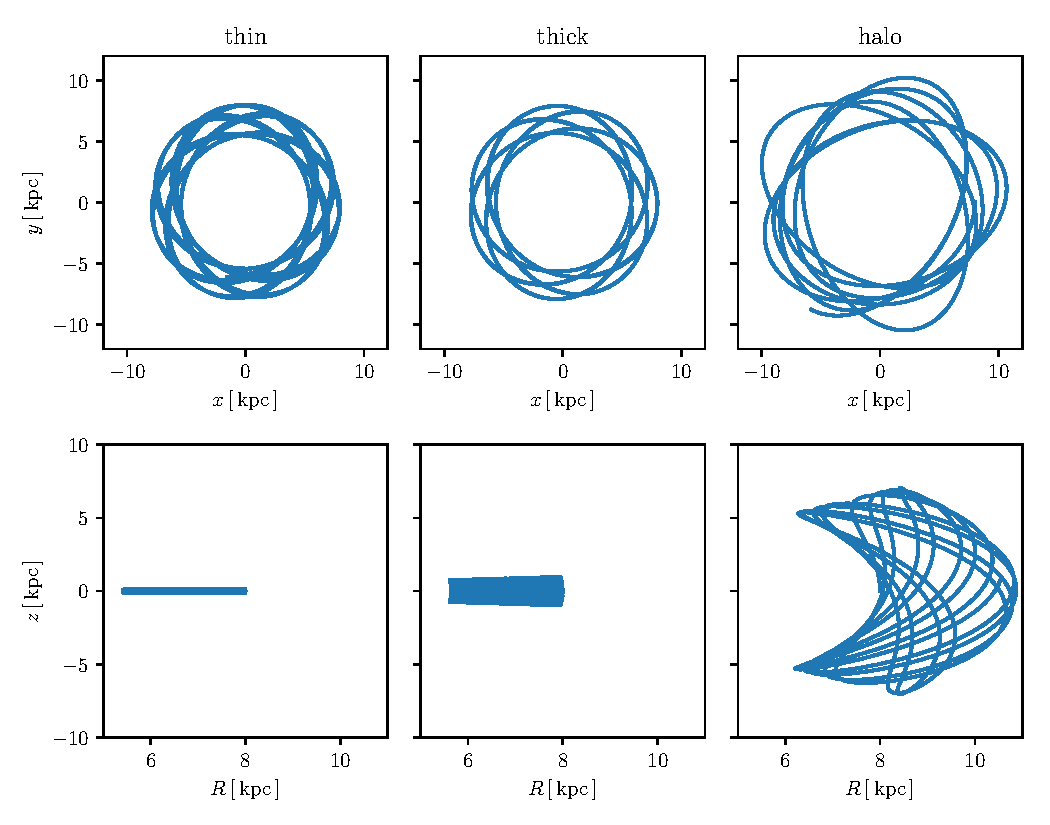
\includegraphics[width=\textwidth]{fig/orbits.pdf}
\end{center}
\caption{The three orbits presented in Table~\ref{tab:orbits} and considered
throughout the work. We plot the thin-disk, thick-disk, and halo orbits in the left, center, and right columns, respectively. The upper
row shows a plot of $x$ vs. $y$ while the lower row shows $R$ vs. $z$.}
\label{fig:plot_orbits}
\end{figure*}

\section{$\Delta R$-$\Delta x$ Relation} \label{app:deltax}
We considered the effect on actions of an inaccuracy in the distance from the
Sun to the Galactic center, which introduces an offset in the $x$ coordinate,
$\Delta x$, of each star when converting to a Galactocentric coordinate
system. In observations of nearby stars, we have that $\Delta x \sim \Delta
R$. However, for the experiment we performed in Section~\ref{ssec:quant} we
considered observations of a star throughout its entire orbit. Therefore, we
must average $\Delta R$ over the course of the orbit. We derive this relation
now.

An offset $\Delta x$ results in an erroneous radius $R_{\text{err}}$ related by
the formula,
\beq
(x+\Delta x)^2 + y^2 = R_{\text{err}}^2\text{.}
\eeq
Keeping only terms to first order in $\Delta x$, we have that,
\beq
\begin{split}
R_{\text{err}}^2 &= R^2 - 2 R \cos{\phi} \Delta x \\
\implies \Delta R &\equiv \abs{R_{\text{err}} - R} 
        = \abs{\cos{\phi}} \Delta x\text{.}
\end{split}
\eeq
Averaging over the circle, we therefore have that,
\beq
\avg{\Delta R} = \frac{2}{\pi} \Delta x\text{.}
\eeq

\section{LSR Variations} \label{app:lsr}
We consider the variations of the LSR as a function of azimuth at the fiducial
solar circle ($R_{0} = 8.2\,\kpc$) in Figure~\ref{fig:lsr_variations}. At
each azimuth, $\phi$, we take the median velocity in cylindrical coordinates
of all stars within $200\,\pc$ of the position, following
\citet{2018arXiv180610564S}. No best-fit subtraction was performed as in
Figure~\ref{fig:midplane}.

\begin{figure*}[htb!]
\begin{center}
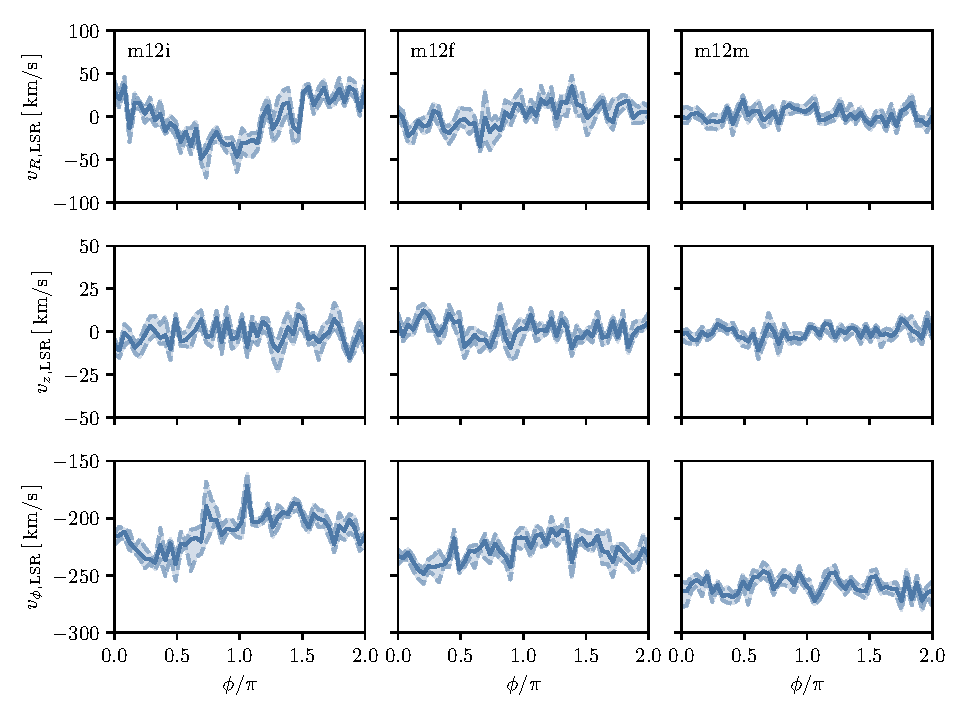
\includegraphics[width=\textwidth]{fig/lsr.pdf}
\end{center}
\caption{The LSR as a function of azimuth at the
fiducial Solar circle ($R_0 = 8.2\,\kpc$). No best-fit subtraction is
performed here as we did in the case of the midplane
(Section~\ref{ssec:local_midplane}). Variations in $v_z$ are on the order of
$\sim5\textup{--}10\,\kms$.}
\label{fig:lsr_variations}
\end{figure*}

\bibliography{references}

\end{document}
